\section{Antenna simulation}
There are some problems with the standard method, so we want to look for a different way to do it.
To start we want to simulate one antenna, that means having a given geometry we want to compute its beam pattern. For that you have the Maxwell equations, but solve them for big antennas at high frequencies will take ages, so we make some compromises.

The idea to simulate the antenna is to start from a known source, illuminate the geometry and compute the reflected field. 
The Kirchhoff-Fresnel equation shown in \ref{eq:kirchhoff_fresnel} is a scalar approximation to compute the reflected field that hits a given geometry. The beuty of this equation is that the incoming wave is reflected in a geometrical way, but each point generates a spherical wave and then you integrate everything. This naturally depicts the diffraction effects that we have in our measurement system.

\begin{equation}
    E_r(\vec{r}) = \frac{-i k}{4\pi}\int E_{i}(\vec{r'})  \frac{e^{ik(|\vec{r}-\vec{r'}|}}{|\vec{r}-\vec{r'}|} \left( \hat{r}\cdot \hat{n} \right) dS
    \label{eq:kirchhoff_fresnel}
\end{equation}

So the main idea is:
\begin{enumerate}
    \item We start from a horn antenna located in the optical path, this antenna emits a know field that we propagate all the way up to the subreflector (that have an hiperboloid geometry)
    \item At the subreflector, we compute the reflected field and propagate it to the primary dish (that ideally has a parabolic geometry).
    \item At the primary, we compute the reflected fields at 1835mts in an area of $3^{\circ}\times 3^{\circ}$ to have the beam map.
\end{enumerate}


\begin{figure}[h]
    \centering
    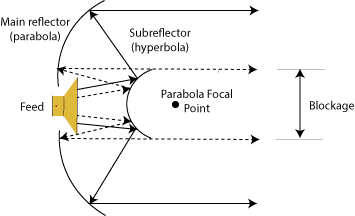
\includegraphics[width=0.5\textwidth]{images/cassegrain_architecture.png}
    \caption{Diagram of the simulation}
    \label{fig:cassegrain_diag}
\end{figure}



\section{Geometry}
Due the problem symetries we take cylindrical parametrization for all the geometries.
Also is good to remember that we are dealing with curved surfaces, so the good orthogonal coordinates rely in the tangent vectors of the surface. In our case those are given by equations \ref{eq:curved_tangent}, with those we can compute the normal vectors as shown in \ref{eq:normal_vector} and the differential surface as \ref{eq:curved_ds}.


\begin{align}
    \vec{t_r} = \frac{\partial \vec{r}}{\partial r} &&  \vec{t_{\phi}} = \frac{\partial \vec{r}}{\partial \phi}
    \label{eq:curved_tangent}
\end{align}

\begin{equation}
    \hat{n} =  \frac{\vec{t}_r \times \vec{t}_{\phi}}{|\vec{t}_r \times \vec{t}_{\phi}|}
    \label{eq:normal_vector}
\end{equation}

\begin{equation}
    dS = \vec{t}_r \times \vec{t}_{\phi}dr d\phi
    \label{eq:curved_ds}
\end{equation}


So now we need to compute all these for the different geometries that we have in the problem.





\subsection{Ideal main dish}
Here we will start with the ideal paraboloid and then introduce the deformation over it.
The ideal paraboloid is given by the equation \ref{eq:perf_parabola} where $f$ is the foci of the parabola.

\begin{equation}
    \vec{S_0}(r, \phi) = \left(r\cos(\phi), r\sin(\phi), \frac{r^2}{4f} \right)
    \label{eq:perf_parabola}
\end{equation}


We build the curved coordinate system with the normalized tangent vectors, they are by construction an orthonormal basis (we will use them later)
\begin{align}
    \hat{e}_{r} = \left( \cos(\phi), \sin(\phi), \frac{r}{2f} \right) \frac{1}{\sqrt{1+\frac{r^2}{4f^2}}} \\
    \hat{e}_{\phi}  = \left(-\sin(\phi), \cos(\phi),0 \right)
\end{align}

The normal vectors are given by 
\begin{equation}
    \hat{n}_0 = \hat{e}_r \times \hat{e}_{\phi} = \left( -\frac{r}{2f} \cos(\phi), -\frac{r}{2f}\sin(\phi), 1 \right) \cdot \frac{1}{\sqrt{1+\frac{r^2}{4f^2}}}
\end{equation}

And the differential surface is given by
\begin{equation}
    dS =  r \sqrt{1+\frac{r^2}{4f^2}} dr d\phi
\end{equation}


\subsection{Deformed main dish}
I just want to start saying that all the expressions here are horrible, but the main idea is simple: we add a deformation pointing in the normal direction of the paraboloid surface. Since each panel is independent we create a local coordinate system for each panel based in the tangent vectors of the ideal paraboloid and we add the deformations there.
The thing is that we need to compute once again the new tanget vectors, normal vectors and the differential surface of the modified paraboloid, which are once again super awfull.



For each panel in the dish we will generate a local coordinate system. 

Once again we return to the panel example image at figure \ref{fig:apex_panel2}, now we will use $(x,y)$ as as the tangent vectors coordinate system as the equations \ref{eq:panel_coord_x} and \ref{eq:panel_coord_y}, where $\vec{p}_{0i}$ is the center of the panel i and $\vec{p_i}$ are the points that belong to that panel.

\begin{equation}
    \vec{x'_i} = \left(\vec{p_i} -\vec{p_{0i}}\right)\cdot \hat{e}_{r}
    \label{eq:panel_coord_x}
\end{equation}

\begin{equation}
    \vec{y'_i} = \left(\vec{p_i} - \vec{p_{0i}}\right)\cdot \hat{e}_{\phi}
    \label{eq:panel_coord_y}
\end{equation}


\begin{figure}[h]
    \centering
    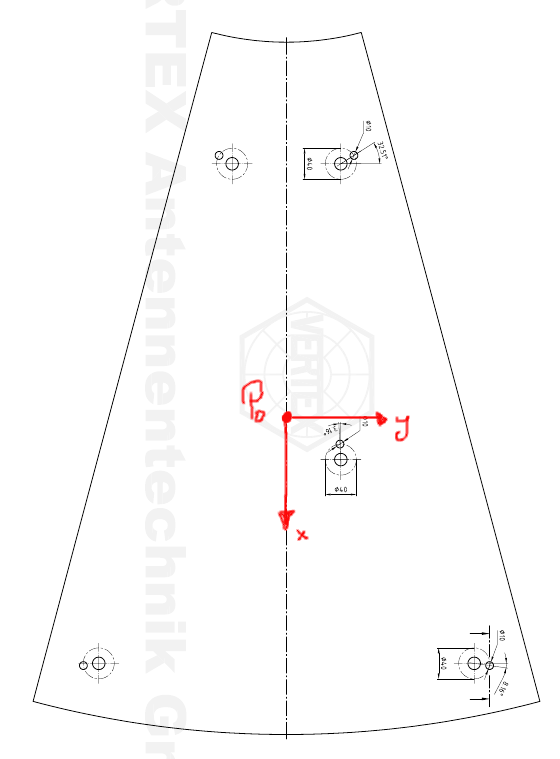
\includegraphics[width=0.3\textwidth, angle=90]{images/apex_panel_diag_coord.png}
    \caption{APEX panel example.}
    \label{fig:apex_panel2}
\end{figure}




With that we can define the modified surface as \ref{eq:modified_surface} where we are adding deformations in the normal direction of the panels with the function $f(x,y, params)$ defined in equation \ref{eq:deformation_func} where $\text{params}_i=\{a_i, b_i, c_i, d_i, e_i\}$ are the parameters that define the deformation of the panel i. The $\delta$ in the equation \ref{eq:modified_surface} is a Kronecker delta that limits the area of the panel i.


\begin{equation}
    \vec{r}_{prim} =\vec{S_{0}}(r,\phi)+\sum_i \left[ f(x'_i, y'_i,\text{params}_i )\cdot \hat{n}_0(r,\phi) \delta({\tiny r_{min,i}<r<r_{max,i}; \phi_{min,i}<\phi<\phi_{max,i}}) \right]
    \label{eq:modified_surface}
\end{equation}

\begin{equation}
    f(x'_i,y'_i, \text{params}_i) = a_i+b_ix'_i+c_iy'_i+d_i({x'}_{i}^2+{y'}_i^2)+e_i({x'}_i^2-{y'}_i^2)
    \label{eq:deformation_func}
\end{equation}


Now we once again need to compute the tangent and normal vectors to get the differential surface of this new surface. 


After some tedious math we arrive to the following representation of the tangent vectors

\begin{equation}
    \partial_r \vec{r}_{prim} =\partial_r S_0 +\frac{\partial f}{\partial x'}\left(\sqrt{1+\frac{r^2}{4f^2}}+(\vec{p}-\vec{p}_0)\cdot \frac{\partial \hat{e}_r}{\partial r} \right)\hat{n}_0+f(x',y')\frac{\partial \hat{n}_0}{\partial r}
\end{equation}

\begin{equation}
    \partial_{\phi}\vec{r}_{prim} = \partial_{\phi} S_0 + \left[ (\vec{p}-\vec{p}_0)\cdot \left( \frac{\partial f}{\partial x'}\frac{\partial \hat{e}_r}{\partial \phi} + \frac{\partial f}{\partial y'} \frac{\partial \hat{e}_\phi}{\partial \phi}\right) +r\frac{\partial f}{\partial y'}\right]\hat{n}_0 + f(x',y')\frac{\partial \hat{n}_0}{\partial \phi}
\end{equation}

And finally we compute the normal vectors as
\begin{equation}
    \vec{n} = \partial_r\vec{r}_{prim}  \times \partial_{\phi}\vec{r}_{prim}
\end{equation}

And build the differential surface as:
\begin{equation}
    dS_{prim} = |\partial_r\vec{r}_{prim}  \times \partial_{\phi}\vec{r}_{prim}| dr d\phi
\end{equation}




\subsection{Hyperboloid}

The subreflector positions are constructed with the equation \ref{eq:hyperboloid_geo} where the hyperboloid parameters are $a,b$.

\begin{equation}
    \vec{r}_{sec} = \left(r\cos(\theta), r\sin(\theta), a \sqrt{\frac{r^2}{b^2-1}}-a  \right)
    \label{eq:hyperboloid_geo}
\end{equation}

The normal vectors are given by \ref{eq:sec_normal} and the differential area by equation \ref{eq:sec_ds}.

\begin{equation}
    \partial z_r = ar/(b^2 \sqrt{r^2/b^2+1})
\end{equation}
\begin{equation}
    \vec{n}_{sec} = \big(-\partial z_r \cos(\phi), -\partial z_r \sin(\phi), 1 \big) \frac{1}{\sqrt{1+(\partial z_r)^2}}
    \label{eq:sec_normal}
\end{equation}


\begin{equation}
    dS_{sec} = r\sqrt{1+(\partial z_r)^2}
    \label{eq:sec_ds}
\end{equation}


\subsection{Horn beam}

Located in the optical path we have a horn antenna, which pattern can be represented by the gaussian beam equations at \ref{eq:gauss_field}. These equations are written in cylindricals, with $z$ pointing outwards the horn antenna. The figure \ref{fig:gauss_beam} shows the beam propagation of the gaussian beam.
Each horn has a parameter $\omega_0$ that is called beam waist, this can be obtained from the geometry of the horn.


The equations look awfull, but if we keep the subreflector and horn at fix postion, we just need to evaluate the function \ref{eq:gauss_field} at the postions $\vec{r}_{sec}$ a single time and then we can reuse it.

\begin{gather}
    z_c = \frac{\pi \omega_0^2}{\lambda}  \\
    \omega(z) = \omega_0 \left[1+ \left(\frac{z}{z_c} \right)^2  \right]^{0.5} \\
    R(z) = z+\frac{z_c^2}{z} \\
    \phi(z) = tan^{-1}(z/z_c )
    \label{eq:gaussian_params}
\end{gather}


\begin{equation}
    E_{horn}(r, z) = \sqrt{ \frac{2}{\pi \omega(z)^2}} exp \left( -\frac{r^2}{\omega(z)^2} -ikz -\frac{i\pi r^2}{\lambda R(z)}+i\phi(z) \right)
    \label{eq:gauss_field}
\end{equation}



\begin{figure}[h]
    \centering
    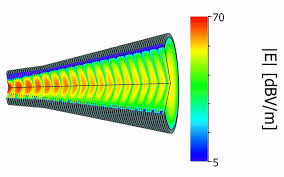
\includegraphics[width=0.3\textwidth]{images/horn_gauss_beam.jpeg}
    \caption{Gaussian beam from a horn.}
    \label{fig:gauss_beam}
\end{figure}



\section{Summary of the antenna simulation}
There are plenty of awfull equations, but in principle we just need to evaluated them in the proper values

\begin{itemize}
    \item If we left the horn and the subreflector at fixed position, then we only need to compute a single time $\vec{r}_{sec}, \hat{n}_{sec}, E_{horn}(\vec{r}_{sec}), dS_{sec}$.
    \item When deforming the primary we will need to update $\vec{r}_{prim}, \hat{n}_{prim}, dS_{prim}$ for the sets $\{a_i, b_i, c_i, d_i, e_i \} i\in \{1,..,265\}$ 
    \item We compute the reflected field of the secondary to the primary positions, for this integral the only thing that may vary between iterations are the $\vec{r}_{prim}$.
        \begin{equation}
            E_{prim}(\vec{r}_{prim}) = \frac{-i k}{4\pi}\int_{r' \in \vec{r}_{sec}} E_{horn}(\vec{r'})  \frac{e^{ik(|\vec{r}_{prim}-\vec{r'}|}}{|\vec{r}_{prim}-\vec{r'}|} \left( \hat{r}_{prim}\cdot \hat{n}_{sec} \right) dS_{sec}
        \end{equation}


    \item We compute the reflected field of the primary to the final positions with the equations.
        \begin{equation}
            E_{final}(\vec{r}_{final}) = \frac{-i k}{4\pi}\int_{r' \in \vec{r}_{prim}} E_{horn}(\vec{r'})  \frac{e^{ik(|\vec{r}_{final}-\vec{r'}|}}{|\vec{r}_{final}-\vec{r'}|} \left( \hat{r}_{final}\cdot \hat{n}_{prim} \right) dS_{prim}
        \end{equation}
\end{itemize}




\section{Optimization}
The final idea of all this development is to introduce a measured beam map and to tell the optimizer "find the set of deformation parameters that generates the most similar beam map to the measured one".


For that we used an adam optimizer with the coefficients $\{a_i, b_i, c_i, d_i, e_i\} i \in \{1,..,265\}$ as parameters to tune (1325 parameters in total) and we use the loss function as the expression in \ref{eq:loss_func} where the regularization parameter is to penalize the surface RMS added via the deformation.

\begin{equation}
    Loss = \sum_{r \in \vec{r}_{final}} (E_{final}(r)-E_{measured}(r))^2 + \lambda \underbrace{\sum_{i} (f(x',y', \text{params}_{i}))^2}_{regularization}
    \label{eq:loss_func}
\end{equation}

We made all the code using the Jax library, then we can rely in the automatic differentiation to make partial derivatives for the deformation coefficients allowing to use gradient descendent optimization.


